% Add "answers" option to print the answers
\documentclass[addpoints]{exam}

\usepackage[utf8]{inputenc}
\usepackage{calc}
\usepackage{listings}
\usepackage{xcolor}
\usepackage{xspace}

\definecolor{codegreen}{rgb}{0,0.6,0}
\definecolor{codegray}{rgb}{0.5,0.5,0.5}
\definecolor{codepurple}{rgb}{0.58,0,0.82}

\lstdefinestyle{Cstyle}{
    commentstyle=\color{codegreen},
    keywordstyle=\color{magenta},
    numberstyle=\tiny\color{codegray},
    stringstyle=\color{codepurple},
    basicstyle=\ttfamily\small,
    breakatwhitespace=true,
    breaklines=true,
    captionpos=b,
    keepspaces=true,
    numbers=left,
    numbersep=5pt,
    showspaces=false,
    showstringspaces=false,
    showtabs=false,
    tabsize=4
}

\lstset{style=Cstyle}

% \makebox[\textwidth]{Name:\enspace\hrulefill}
%
% \vspace{5mm}
%\makebox[\textwidth]{Instructor’s name:\enspace\hrulefill}

\newcommand{\truefalse}
{		\begin{checkboxes}
			 \choice True
			 \choice False. Explanation:
		\end{checkboxes}
		\vspace{10pt}
}

\newcommand{\answerspace}[1]
{
	\ifprintanswers
	\else
		\setlength{\mylength}{10pt}%
		%\noindent\rule{\mylength}{20pt}
		%\vspace{\fpeval{1.2*(#1)}}
		\vspace{#1\mylength}
	\fi
}
\newlength{\mylength}

\newcommand\pf[1]{\textcolor{red}{PF: #1}}
\newcommand\am[1]{\textcolor{blue}{AM: #1}}

\newcommand{\answer}[1]{\begin{solution}{#1}\end{solution}}
\newcommand{\ra}{$\rightarrow$\xspace}


\usepackage{color}
\usepackage{lastpage}
\usepackage{verbatim}
\usepackage{fancyvrb}
\usepackage{graphicx}
\usepackage{float}
\usepackage{minted}
\usepackage{multicol}
\usepackage{amsmath}
\usepackage{amssymb}

\usepackage[svgnames]{xcolor}
\usepackage[colorlinks=true, allcolors=MidnightBlue]{hyperref}

% For those sweet, sweet acmart fonts.
\usepackage[T1]{fontenc}
\usepackage[tt=false, type1=true]{libertine}
\usepackage[varqu]{zi4}                  % Inconsolata for \ttfamily

% Eliminate extraneous spacing on itemize, description, etc.
\usepackage{enumitem}
\setlist{nosep}

\newcommand{\Code}[1]{\mintinline{python}{#1}}
\newcommand{\nonAnswerNewPage}{\ifprintanswers \vfill \else \newpage \fi}

% Macro for lockset answers
\newcommand{\LS}[1]{\texttt{\{#1\}}}

% Macro for sign-analysis abstract values
\newcommand{\Neg}{\textsf{neg}}
\newcommand{\Zero}{\textsf{zero}}
\newcommand{\Pos}{\textsf{pos}}
\newcommand{\NonZero}{\textsf{nonzero}}

\renewcommand{\solutiontitle}{\noindent\textbf{Solution sketch: }}
\definecolor{SolutionColor}{rgb}{0.8,0.9,1}

%Tikz nonsense for the Hasse diagram
\usepackage{tikz}
\usepackage{amsmath}
\usetikzlibrary{positioning}

\cfoot{Page \thepage\ of \pageref{LastPage}}
\rhead{Initials: \rule{20mm}{0.4pt}}

%%%%%%%%%%%%%%%%%%%%%%%%%%%%%%%%%%%%%%%%
\begin{document}
\fvset{numbers=left,numbersep=3pt}
\thispagestyle{empty}

\begin{center}
  {\LARGE{\textbf{CS 408: Homework 6}}}\\
  \vspace*{5pt}
  {\Large Deadline: Friday, December 4 \textbf{at 6PM}}\\
  \vspace*{10pt}

  \fbox{
    \fbox{\parbox{6in}{\centering
        \begin{itemize}
        \item The homework is open notes, open book.
        \item Please upload an annotated version of this pdf, ensuring
          that each answer fits in the box following each question.
        \item All solutions must be \textbf{handwritten}; typed work
          will not receive any credit. You may annotate the pdf
          directly, no need to print out and rescan.
        \item No AI tools allowed.
        \item No collaboration with your peers of any kind allowed on
          this homework.
        \item Homeworks are due at \textbf{6PM}. Anything submitted
          after \textbf{6PM} will not be accepted.
        \item Provide complete and clear but concise answers. Clearly
          explain your answers where required.
	\end{itemize}
      }}}
\end{center}

\begin{center}
	\makebox[0.6\textwidth]{
		\combinedgradetable[h][questions]
	}
\end{center}
%\begin{center}\combinedgradetable[h][questions]\end{center}

\vspace{5mm}
\begin{center}
\makebox[\textwidth]{\textbf{Name (please print)}: \rule{100mm}{0.8pt} }
\end{center}

\begin{questions}

%% =====================================================================
%% Q1 -- REGRESSION TEST SELECTION  (safe vs. precise)
%% =====================================================================
\question Suppose we are maintaining a super popular open source
  project, \textsf{Shapes++}, that contains three functions and a
  suite of five regression tests. The table below records which
  functions each test executes:

  \begin{center}
    \begin{tabular}{ll}
      test & functions executed \\ \hline
      \Code{t1} & \Code{area} \\
      \Code{t2} & \Code{perimeter} \\
      \Code{t3} & \Code{describe} \\
      \Code{t4} & \Code{area}, \Code{perimeter} \\
      \Code{t5} & \Code{area}, \Code{describe} \\
    \end{tabular}
  \end{center}

  A contributor has submitted a pull request that modifies \Code{area}
  so that it rejects a negative width:
\begin{minted}{python}
# before                          # after
def area(w, h):                   def area(w, h):
    return w * h                      if w < 0:
                                          raise ValueError
                                      return w * h
\end{minted}
  \noindent Suppose that running this test suite is quite expensive,
  so we use a smart continuous integration mechanism to avoid running
  the entire test suite each time a pull request is submitted.
\begin{parts}

\part[2] A regression test selection technique is said to be
  \textbf{safe} if it never omits a test whose result could be
  affected by the change. Based on the table above, which tests would
  our CI run if it implemented a safe test selection strategy?
  \begin{solutionorbox}[1.2in]
    \Code{t1}, \Code{t4} and \Code{t5} --- every test that executes
    \Code{area}. A safe technique has only the dependency information
    to go on, so it must select all three.
  \end{solutionorbox}

\nonAnswerNewPage

\part[2] Now suppose the three tests call \Code{area} with the
  following arguments:

  \begin{center}
    \begin{tabular}{ll}
      test & call \\ \hline
      \Code{t1} & \Code{area(3, 4)} \\
      \Code{t4} & \Code{area(-1, 5)} \\
      \Code{t5} & \Code{area(2, 2)} \\
    \end{tabular}
  \end{center}

  A regression test selection technique is \textbf{precise} if it
  never selects a test whose result is unaffected by the change. Which
  tests would our CI run if it implemented a precise selection
  strategy? If that set is different from your previous answer,
  explain why.
  \begin{solutionorbox}[2in]
    Only \Code{t4}. The change affects \Code{area} only when
    \Code{w < 0}, and \Code{t4} is the only test that calls it with a
    negative width: it used to return $-5$ and now raises
    \Code{ValueError}. \Code{t1} and \Code{t5} still compute
    \Code{12} and \Code{4} exactly as before.

    The safe technique selected \Code{t1} and \Code{t5} unnecessarily.
    They are \emph{false selections}: wasted machine time, but not
    wrong answers.
  \end{solutionorbox}

\part[4] Explain why, in general, no regression test selection
  technique can be both safe and precise. Which strategy should our CI
  pick, and why?
  \begin{solutionorbox}[3in]
    To be precise, a technique would have to decide \emph{in advance}
    whether a change alters a given test's result --- which amounts to
    predicting the test's outcome without running it. That is
    undecidable in general: it would require deciding whether two
    programs agree on a given input, and the modified code may not even
    terminate.

    So a technique can be safe (select too much) or precise (risk
    selecting too little), but not reliably both. Real tools choose
    \textbf{safety}, because the two failure modes are not
    symmetrical. An imprecise technique costs machine time, which is
    cheap and getting cheaper. An unsafe technique silently skips the
    one test that would have caught a regression --- and the whole
    point of a regression suite is that it does not do that.

    (This is the same asymmetry we see with the lockset algorithm,
    which also prefers reporting too much to reporting too little.)
  \end{solutionorbox}

\end{parts}

\nonAnswerNewPage

%% =====================================================================
%% Q2 -- TEST CASE PRIORITIZATION
%% =====================================================================
\question Suppose \textsf{Shapes++} has an additional test suite which
  covers five test requirements. The table below reports which
  requirements each test covers:

  \begin{center}
    \begin{tabular}{ll}
      test & requirements covered \\ \hline
      \Code{t1} & 1, 2, 3 \\
      \Code{t2} & 1, 2, 4 \\
      \Code{t3} & 5 \\
      \Code{t4} & 3, 4, 5 \\
    \end{tabular}
  \end{center}

  Now, suppose our goal is for our CI mechanism to \textbf{prioritize}
  this suite, i.e., it \textbf{always} run these four tests, but tries
  to do so in an order that satisfies as many requirements as early as
  possible.

\begin{parts}

\part[2] The \textbf{total greedy} heuristic orders tests by how many
  requirements each one covers, starting with the test that covers the
  most, breaking ties by test number. What order does this heuristic
  produce, and how many requirements have been covered after each
  test?
  \begin{solutionorbox}[2in]
    \Code{t1} (3), \Code{t2} (3), \Code{t4} (3), \Code{t3} (1), with
    the three-way tie broken by test number:
    \begin{center}
      \Code{t1}, \Code{t2}, \Code{t4}, \Code{t3}
    \end{center}
    Cumulative coverage: $3, 4, 5, 5$.
  \end{solutionorbox}

\part[2] The \textbf{additional greedy} heuristic repeatedly picks the
  test covering the most requirements \emph{not yet covered by the
    tests already chosen}. What order does this strategy produce, and
  how many requirements have been covered after each test?
  \begin{solutionorbox}[2in]
    \Code{t1} covers 3 new requirements, more than any other test, so
    it goes first; that covers $\{1, 2, 3\}$.

    Of what remains, \Code{t2} adds only $\{4\}$ and \Code{t3} only
    $\{5\}$, but \Code{t4} adds both $\{4, 5\}$ --- so \Code{t4} goes
    second. Everything is now covered, and the remaining two tests
    follow in any order:
    \begin{center}
      \Code{t1}, \Code{t4}, \Code{t2}, \Code{t3}
    \end{center}
    Cumulative coverage: $3, 5, 5, 5$.
  \end{solutionorbox}

\nonAnswerNewPage

\part[4] Which ordering heursitic should our CI system adopt? Given
  that it runs all four tests regardless, what do we gain by bothering
  with prioritizing those tests, as opposed to, say running them in an
  arbitrary order?
  \begin{solutionorbox}[2.5in]
    Additional greedy is better: it covers all five requirements after
    two tests, where total greedy needs three. \Code{t2} looks
    attractive to total greedy because it covers three requirements,
    but two of them were already covered by \Code{t1}.

    Prioritization does not make the suite faster or smaller --- every
    test still runs. What it buys is \textbf{earlier feedback}: if the
    suite is cut short by a timeout, or a developer is watching the
    first few results, the most informative tests have already run. On
    a suite that takes hours, that is the difference between learning
    about a failure in minutes and learning about it after lunch.
  \end{solutionorbox}

\end{parts}

\nonAnswerNewPage

%% =====================================================================
%% Q3 -- LOCKSET ANALYSIS
%% =====================================================================
\question Consider the following program:

\begin{minted}{c}
int x = 0;
pthread_mutex_t A;

void *T1(void *arg) {
    pthread_mutex_lock(&A);
    x = 1;
    pthread_mutex_unlock(&A);
    return NULL;
}

void *T2(void *arg) {
    x = 2;
    return NULL;
}
\end{minted}

  Suppose this program executes according to the following schedule:
  \begin{enumerate}
  \item \textbf{T1:} L(A)
  \item \textbf{T2:} W(x)
  \item \textbf{T1:} W(x)
  \item \textbf{T1:} U(A)
  \end{enumerate}

  \textbf{Answer format:} Write $C(\texttt{x})$ for the candidate
  lockset of the shared variable \texttt{x}, and write $H(T)$ for the
  set of locks held by thread $T$. Give every lockset in curly braces
  (\texttt{\{\}}), e.g.\ \LS{} (the empty set), \LS{A}, \LS{A, B}. Do
  not write \texttt{None}, \texttt{empty}, or leave the text field
  empty.

  \begin{parts}

  \part[1] Which locks are held by \textbf{T2} when it performs step 2?
    \begin{solutionorbox}[.5in]
      \LS{}
    \end{solutionorbox}

  \part[1] What is $C(\texttt{x})$ after step 2?
    \begin{solutionorbox}[.5in]
      \LS{}
    \end{solutionorbox}

  \part[1] Which locks are held by \textbf{T1} when it performs step 3?
    \begin{solutionorbox}[.5in]
      \LS{A}
    \end{solutionorbox}

  \part[1] What is $C(\texttt{x})$ after step 3?
    \begin{solutionorbox}[.5in]
      \LS{}
    \end{solutionorbox}

  \part[1] Does the lockset race algorithm report a potential data race
    on this execution? Explain.
    \begin{solutionorbox}[.5in]
    Yes. $C(\texttt{x})$ is empty after step 3, so the lockset algorithm flags a
      potential race.
    \end{solutionorbox}

    \nonAnswerNewPage

  \part[2] Is this an actual race? Explain.
    \begin{solutionorbox}[1in]
      Yes. T2 writes to \texttt{x} without holding \texttt{A},
      while T1 writes to \texttt{x} while holding \texttt{A}. The two
      writes are unordered, so this is a genuine data race.
  \end{solutionorbox}
  \end{parts}

  \nonAnswerNewPage

%% =====================================================================
%% Q4 -- LOCKSET ANALYSIS
%% =====================================================================

\question Now consider this program:

\begin{minted}{c}
int x = 0;

void *Worker(void *arg) {
    x = 1;
    return NULL;
}

int main(void) {
    pthread_t t;
    pthread_create(&t, NULL, Worker, NULL);
    pthread_join(t, NULL);
    printf("%d\n", x);
    return 0;
}
\end{minted}

  Suppose this program executes according to the following schedule:
  \begin{enumerate}
  \item \textbf{Main:} \texttt{pthread\_create(Worker)}
  \item \textbf{Worker:} W(x)
  \item \textbf{Worker:} finishes
  \item \textbf{Main:} \texttt{pthread\_join} returns
  \item \textbf{Main:} R(x)
  \end{enumerate}

\begin{parts}

\part[1] Which locks are held by \textbf{Worker} when it performs step 2?
    \begin{solutionorbox}[.5in]
      \LS{}
    \end{solutionorbox}

\part[1] What is $C(\texttt{x})$ after step 2?
    \begin{solutionorbox}[.5in]
      \LS{}
    \end{solutionorbox}

\part[1] Which locks are held by \textbf{Main} when it performs step 5?
    \begin{solutionorbox}[.5in]
      \LS{}
    \end{solutionorbox}

\part[1] What is $C(\texttt{x})$ after step 5?
    \begin{solutionorbox}[.5in]
      \LS{}
    \end{solutionorbox}

\nonAnswerNewPage

\part[2] Does the lockset race algorithm report a potential data race
  on this execution? Explain.
    \begin{solutionorbox}[2.5in]
      Yes. $C(\texttt{x})$ is empty after step 5, so the lockset algorithm flags a
    potential race.
  \end{solutionorbox}

\part[2] Is this an actual race? Explain.
    \begin{solutionorbox}[3.5in]
      No. The \texttt{pthread\_join} guarantees that the worker
      finishes before the main thread reads \texttt{x}, so the two
      accesses are ordered by happens-before. The lockset algorithm
      reports a \emph{false positive} here, because it tracks only locks
      and is blind to the ordering that \texttt{join} establishes.
  \end{solutionorbox}
\end{parts}

\nonAnswerNewPage

%% =====================================================================
%% Q5 -- LOCKSET ANALYSIS, two locks
%% =====================================================================
\question Now consider this program, which uses two locks:

\begin{minted}{c}
int x = 0;
pthread_mutex_t A, B;

void *T1(void *arg) {
    pthread_mutex_lock(&A);
    pthread_mutex_lock(&B);
    x = 1;
    pthread_mutex_unlock(&B);
    pthread_mutex_unlock(&A);
    return NULL;
}

void *T2(void *arg) {
    pthread_mutex_lock(&A);
    x = 2;
    pthread_mutex_unlock(&A);
    return NULL;
}
\end{minted}

  Suppose this program executes according to the following schedule:
  \begin{enumerate}
  \item \textbf{T1:} L(A)
  \item \textbf{T1:} L(B)
  \item \textbf{T1:} W(x)
  \item \textbf{T1:} U(B)
  \item \textbf{T1:} U(A)
  \item \textbf{T2:} L(A)
  \item \textbf{T2:} W(x)
  \item \textbf{T2:} U(A)
  \end{enumerate}

  \begin{parts}

  \part[1] Which locks are held by \textbf{T1} when it performs step 3?
    \begin{solutionorbox}[.5in]
      \LS{A, B}
    \end{solutionorbox}

  \part[1] What is $C(\texttt{x})$ after step 3?
    \begin{solutionorbox}[.5in]
      \LS{A, B}

      This is the first access to \texttt{x}, so $C(\texttt{x})$ is
      narrowed from every lock in the program to exactly the locks T1
      holds.
    \end{solutionorbox}

  \part[1] Which locks are held by \textbf{T2} when it performs step 7?
    \begin{solutionorbox}[.5in]
      \LS{A}
    \end{solutionorbox}

  \part[1] What is $C(\texttt{x})$ after step 7?
    \begin{solutionorbox}[.5in]
      \LS{A}

      $C(\texttt{x})$ is intersected with the locks T2 holds:
      \LS{A, B} $\cap$ \LS{A} $=$ \LS{A}.
    \end{solutionorbox}

    \nonAnswerNewPage
  \part[2] Does the lockset race algorithm report a potential data race
    on this execution? Explain.
    \begin{solutionorbox}[2.5in]
      No. $C(\texttt{x})$ is still non-empty after every access,
      so there is at least one lock --- namely \texttt{A} --- that was
      held on every access to \texttt{x}. The algorithm concludes that
      \texttt{A} consistently protects \texttt{x} and reports nothing.
    \end{solutionorbox}

  \part[2] Suppose T2 acquired a \emph{third} lock \texttt{C} instead
    of \texttt{A}. What would $C(\texttt{x})$ be after step 7,
    and would the algorithm report a race? Explain.
    \begin{solutionorbox}[3.5in]
      $C(\texttt{x})$ would become \LS{A, B} $\cap$ \LS{C} $=$ \LS{},
      and the algorithm \emph{would} report a potential race.

      This would also be a real race: T1 and T2 write to \texttt{x}
      while holding disjoint sets of locks, so nothing prevents the two
      writes from interleaving.
    \end{solutionorbox}

  \end{parts}

\nonAnswerNewPage

%% =====================================================================
%% Q6 -- LOCKSET IS A DYNAMIC ANALYSIS
%% =====================================================================
\question Consider one last program. Here the thread \texttt{T1} tries
  to take the lock, but gives up and writes anyway if it cannot get
  it:\footnote{N.b. \Code{pthread_mutex_trylock} returns \Code{0} if it
    acquired the lock, and a non-zero error code if the lock was
    already held by somebody else.}

\begin{minted}{c}
int x = 0;
pthread_mutex_t A;

void *T1(void *arg) {                 void *T2(void *arg) {
    if (pthread_mutex_trylock(&A)         pthread_mutex_lock(&A);
          == 0) {                         x = 2;
        x = 1;                            pthread_mutex_unlock(&A);
        pthread_mutex_unlock(&A);         return NULL;
    } else {                          }
        x = 1;
    }
}
\end{minted}

  \begin{parts}

  \part[2] Suppose the program executes according to this schedule:
    \begin{enumerate}
    \item \textbf{T1:} L(A) \quad (the \texttt{trylock} succeeds)
    \item \textbf{T1:} W(x)
    \item \textbf{T1:} U(A)
    \item \textbf{T2:} L(A)
    \item \textbf{T2:} W(x)
    \item \textbf{T2:} U(A)
    \end{enumerate}
    What is $C(\texttt{x})$ at the end of this execution, and does the
    lockset algorithm report a race?
    \begin{solutionorbox}[1.2in]
      $C(\texttt{x}) = $ \LS{A}, and \textbf{no race is reported}.
      Both writes happened while holding \texttt{A}, so the
      intersection never empties.
    \end{solutionorbox}

  \part[2] Now suppose the program executes according to this
    schedule instead:
    \begin{enumerate}
    \item \textbf{T2:} L(A)
    \item \textbf{T1:} W(x) \quad (the \texttt{trylock} failed)
    \item \textbf{T2:} W(x)
    \item \textbf{T2:} U(A)
    \end{enumerate}
    What is $C(\texttt{x})$ at the end of this execution, and does the
    lockset algorithm report a race?
    \begin{solutionorbox}[1.2in]
      $C(\texttt{x}) = $ \LS{}, and the algorithm \textbf{does} report
      a race. Because \texttt{T2} already held \texttt{A}, the
      \texttt{trylock} failed and \texttt{T1} took the \Code{else}
      branch, writing to \texttt{x} while holding no locks at all.
    \end{solutionorbox}

  \nonAnswerNewPage

\part[4] Observe that the two schedules above run the \emph{same
    program on the same input}, and yet the algorithm reports a race
  on one and not the other. What does this tells us about lockset
  analysis and the guarantees it provides?
    \begin{solutionorbox}[2.5in]
      Lockset analysis is a \textbf{dynamic} analysis: it only ever
      sees the instructions that an execution actually performed. The
      unlocked write in the \Code{else} branch is a bug in the program
      whichever way it runs --- but the analysis can only observe it
      on a schedule where the \texttt{trylock} fails, and that depends
      entirely on the timing of the two threads.

      So a clean report means only ``no race was witnessed on the
      schedules I happened to run.'' It is \emph{not} a proof that the
      program is race-free. In practice this is why race detectors are
      run over large test suites, often with a scheduler that
      deliberately perturbs the interleaving, and why a clean run is
      much weaker evidence than it looks.

      (Note that this is a different limitation from the one we saw
      earlier with \texttt{pthread\_join}. There, the algorithm saw
      everything it needed and still reported a \emph{false positive}.
      Here, the algorithm is simply never shown the problem.)
    \end{solutionorbox}

  \end{parts}

  \nonAnswerNewPage

%% =====================================================================
%% Q7 -- SIGN ANALYSIS  (apply an analysis from class)
%% =====================================================================
\question Recall the \textbf{sign analysis} we saw in class, whose
  abstract values are:

  \begin{center}
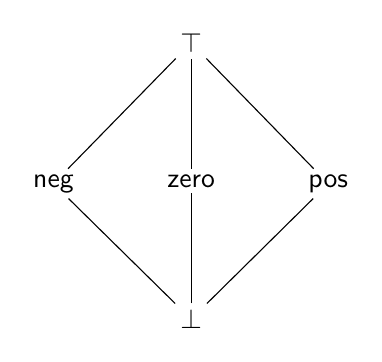
\begin{tikzpicture}[
  every node/.style={inner sep=2pt},
  node distance=14mm and 12mm
]
\node (top)  {$\top$};
\node (neg)  [below left=of top]  {$\Neg$};
\node (zero) [below=of top]       {$\Zero$};
\node (pos)  [below right=of top] {$\Pos$};
\node (bot)  [below=14mm of zero] {$\bot$};

\draw (bot) -- (neg);
\draw (bot) -- (zero);
\draw (bot) -- (pos);
\draw (neg) -- (top);
\draw (zero) -- (top);
\draw (pos) -- (top);
\end{tikzpicture}
\end{center}

\noindent where \Neg{} means ``definitely negative'', \Zero{} means
  ``definitely zero'', \Pos{} means ``definitely positive'', $\bot$
  means ``no value reaches this point'', and $\top$ means ``could be
  anything''.

  Consider the following program:

\begin{minted}{python}
def f(n: int) -> int:
    x = 0
    if n > 0:
        x = 1
    else:
        x = -1
    y = 10 // x
    return y
\end{minted}

\begin{parts}

\part[6] Apply the path-insensitive, forward data-flow analysis
  algorithm from class to this program. Give your answer as a CFG in
  which each node is annotated with an input abstract state, a basic
  block or conditional identifier, and an output abstract state.
  \begin{solutionorbox}[4in]
    \begin{center}\small
      \begin{tabular}{llll}
        node & in & & out \\ \hline
        \Code{L2: x = 0}      & [\Code{n}$\mapsto\top$, \Code{x}$\mapsto\bot$, \Code{y}$\mapsto\bot$]  && [\Code{n}$\mapsto\top$, \Code{x}$\mapsto\Zero$, \Code{y}$\mapsto\bot$] \\
        \Code{C3: n > 0}      & [\Code{n}$\mapsto\top$, \Code{x}$\mapsto\Zero$, \Code{y}$\mapsto\bot$] && unchanged \\
        \Code{L4: x = 1}      & [\Code{n}$\mapsto\top$, \Code{x}$\mapsto\Zero$, \Code{y}$\mapsto\bot$] && [\Code{n}$\mapsto\top$, \Code{x}$\mapsto\Pos$, \Code{y}$\mapsto\bot$] \\
        \Code{L6: x = -1}     & [\Code{n}$\mapsto\top$, \Code{x}$\mapsto\Zero$, \Code{y}$\mapsto\bot$] && [\Code{n}$\mapsto\top$, \Code{x}$\mapsto\Neg$, \Code{y}$\mapsto\bot$] \\
        \Code{L7: y = 10//x}  & [\Code{n}$\mapsto\top$, \Code{x}$\mapsto\top$, \Code{y}$\mapsto\bot$]  && [\Code{n}$\mapsto\top$, \Code{x}$\mapsto\top$, \Code{y}$\mapsto\top$] \\
      \end{tabular}
    \end{center}

    The important step is the \textbf{join} before line 7, where the
    two branches meet:
    \[
      \Pos \sqcup \Neg \;=\; \top
    \]
    so \Code{x} enters line 7 as $\top$.
  \end{solutionorbox}

\nonAnswerNewPage

\part[2] Line 7 divides by \Code{x}. Based on your answer above, does
  this analysis report a possible division by zero?
  \begin{solutionorbox}[1.2in]
    Yes. On entry to line 7 the analysis has \Code{x}$\mapsto\top$, and
    $\top$ includes zero, so it cannot rule out a division by zero and
    must report a possible error.
  \end{solutionorbox}

\part[4] Is there actually an execution of this program that divides by
  zero? Explain.
  \begin{solutionorbox}[1.5in]
    No. Every execution takes one of the two branches, so \Code{x} is
    either \Code{1} or \Code{-1} when line 7 runs --- never \Code{0}.
    The initial \Code{x = 0} on line 2 is always overwritten before it
    is used.

    The report is therefore a \textbf{false positive}.
  \end{solutionorbox}

\part[2] Explain what caused the spurious report. Can you think of a
  change to the set of abstract values that would let the analysis
  prove this division safe?
  \begin{solutionorbox}[3in]
    The join is what loses the information. \Pos{} and \Neg{} have no
    common upper bound in this lattice other than $\top$, so the moment
    the two branches meet, everything the analysis knew about \Code{x}
    --- including the fact that it is not zero --- is discarded.

    Adding an abstract value for ``definitely not zero'' fixes it.
    With \NonZero{} placed between $\{\Neg, \Pos\}$ and $\top$, we get
    \[
      \Pos \sqcup \Neg \;=\; \NonZero
    \]
    and the analysis can prove the division safe. (Lattices used in
    practice usually add \Code{<= 0} and \Code{>= 0} for the same
    reason: each one records a fact that survives a join which would
    otherwise collapse to $\top$.)

    More generally, this is the central trade-off of static analysis:
    a coarser abstraction is cheaper to compute but produces more false
    positives, and a richer one is more precise but more expensive.
  \end{solutionorbox}

\end{parts}

\nonAnswerNewPage

%% =====================================================================
%% Q8 -- STATIC ANALYSIS       [adapted from Spring 2026 HW5, Q4]
%% =====================================================================
\question Consider a program in which each assignment statement is
  labelled by its line number. In the following program, for example,
  \Code{x = 1} is labelled with $1$ and \Code{x = 3} is labelled with
  $4$:

\begin{minted}{python}
x = 1
y = 2
if x > 0:
    x = 3
else:
    y = 4
z = x + y
\end{minted}

  The goal of \textbf{reaching definitions} analysis is to identify, at
  each program point, the set of definitions for each variable that may
  \emph{reach} that point.

  \textbf{Note}: This problem is strictly \textit{optional}!

\begin{parts}

\part[6] Define a set of abstract values that could be used for
  reaching definitions analysis. For each abstract value (or group of
  abstract values), describe what it intuitively represents. Your
  answer should have a similar format to what we saw in class, e.g.
  ``[\Code{x}$\mapsto$c]: the variable \Code{x} has the property
  \ldots''. You should also define an ordering relation on this set.
  (Hint: a Hasse diagram might not be the best way to present your
  ordering here.)
  \begin{solutionorbox}[4in]
    The abstract values are sets of line numbers, i.e.\
    $\mathcal{P}(\mathbb{N})$. Each value represents all of the lines
    holding a definition that \emph{may} reach the current program
    point. So the abstract state [\Code{q}$\mapsto\{1, 5, 6\}$] means
    that at this program point \Code{q} might hold the value assigned
    at line 1, or at line 5, or at line 6, and \emph{cannot} hold a
    value assigned anywhere else.

    The ordering relation is subset inclusion $\subseteq$, with
    $\top = \mathbb{N}$ and $\bot = \emptyset$.
\end{solutionorbox}

\nonAnswerNewPage

\part[6] For the two categories of statement below, define the
  transfer function for this analysis:
  \begin{itemize}
  \item \textbf{Assignment:} \Code{n: x = e}
  \item \textbf{Conditional:} \Code{n: if e1: s2 else: s3}
  \end{itemize}
  (Assume both kinds of statement are labelled with line numbers.)
  Define your transfer functions by showing how each statement
  transforms an abstract state containing three variables \Code{x},
  \Code{y} and \Code{z}, using the format
  \begin{itemize}
  \item transfer([\Code{x}$\mapsto$a, \Code{y}$\mapsto$b,
    \Code{z}$\mapsto$c], \Code{m: x = e}) $\equiv$
    [\Code{x}$\mapsto$d, \Code{y}$\mapsto$e, \Code{z}$\mapsto$f]
  \end{itemize}
  where a, b, c and so on are drawn from the set of abstract values
  you defined in part (a).
  \begin{solutionorbox}[4in]
    \begin{itemize}
    \item transfer([\Code{x}$\mapsto$a, \Code{y}$\mapsto$b,
      \Code{z}$\mapsto$c], \Code{m: x = e}) $\equiv$
      [\Code{x}$\mapsto\{m\}$, \Code{y}$\mapsto$b,
      \Code{z}$\mapsto$c]

      An assignment \emph{kills} every definition of \Code{x} that
      reached this point and \emph{generates} a single new one at line
      $m$; the other variables are untouched.
    \item transfer([\Code{x}$\mapsto$a, \Code{y}$\mapsto$b,
      \Code{z}$\mapsto$c], \Code{m: if e1: s2 else: s3}) $\equiv$
      [\Code{x}$\mapsto$a, \Code{y}$\mapsto$b, \Code{z}$\mapsto$c]

      A conditional assigns nothing, so it neither kills nor generates
      any definition; the abstract state passes through unchanged.
    \end{itemize}
  \end{solutionorbox}

  \nonAnswerNewPage

\part[10] Using your answers from parts (a) and (b), show the CFG that
  results from applying the path-insensitive, forward data-flow
  analysis algorithm discussed in class to the program above. Your
  final answer should be given in the form of a CFG in which each node
  is annotated with an input abstract state, a basic block or
  conditional identifier, and an output abstract state.
  \begin{solutionorbox}[7in]
    %\includegraphics[width=.75\linewidth]{hw6/q3_cfg.png}
  \end{solutionorbox}

\end{parts}

\end{questions}
\end{document}
